\documentclass[letterpaper,12pt]{article}
\usepackage[margin=1in]{geometry}
\usepackage{graphicx}  % Include figure files
\usepackage{xcolor}  % Allow for a color text
\usepackage{amsmath}  % math fonts
\usepackage{amsfonts}  % math fonts
\usepackage{latexsym}  % math fonts
\usepackage{amssymb}  % math fonts
\usepackage{mathtools} % Give more control of how equations are displayed
\usepackage{appendix} % Lets you create an appendix
\usepackage[numbered]{matlab-prettifier} % Let's me import MATLAB code in a nice format
\usepackage{indentfirst} % This indents the first paragraph. By default latex won't do it.
\usepackage{subfigure}

%\setlength{\parskip}{1em} % This skips a line when making new paragraphs
\newtagform{show_eq}{(Eq.\ }{)}  % how the equation numbers are displayed
\usetagform{show_eq} % this goes with the \newtagform

\begin{document}

% ================================== Title Page ==========================================
\begin{titlepage}
 \begin{center}
 \vspace*{1in}
{\Huge Comparison Between Linear and Nonlinear Models for Electro-Mechanical System}\\
    \bigskip
    by\\
    \bigskip
    {\Large Kevin Moran} \\
    \bigskip
    Date : November 15th, 2020

    \bigskip\bigskip\bigskip
    University of Southern California\\
    Aerospace and Mechanical Engineering Department\\
    AME 302 : System Dynamics
 \end{center}
\end{titlepage}

% ================================== Main Text =====================================

\section{State Representation for Coupled System}
Deriving the equation of motion for the motor shown in Figure \ref{motor} yields the equation of motion for the mechanical and electrical systems as :  

\begin{equation}
    J_m\dot{\omega} + b_m\omega = T - T_L= T_m\\
    \label{mechEOM}
\end{equation}

\begin{equation}
    R_fi_f + L_f\frac{di_f}{dt}=e_{f}(t)
    \label{elecEOM}
\end{equation}
    
\begin{figure}[h]
    \centering
    \subfigure[DC Motor : Mechanical]{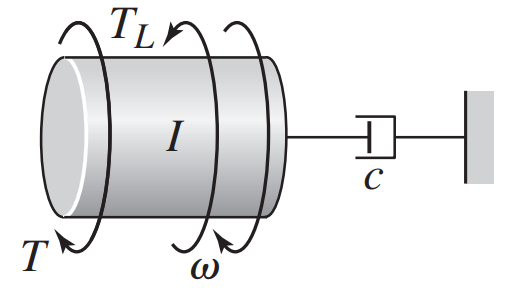
\includegraphics[width=.4\linewidth]{motor.PNG}
    \label{mech}}
    \quad
    \subfigure[DC Motor : Field Circuit]{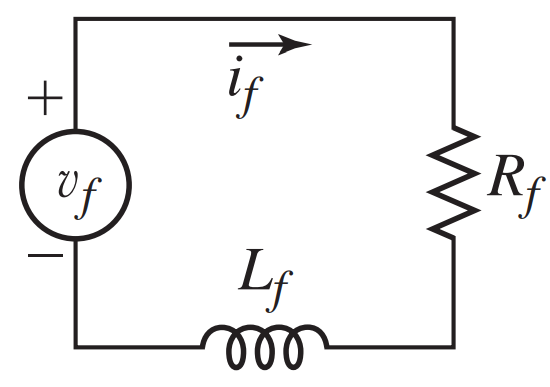
\includegraphics[width=.35\linewidth]{fieldCircuit.PNG}
    \label{circuit}}
    \label{motor}
    \caption{DC Motor shown as a mechanical and electrical system}
\end{figure}

By making the assumptions $R_f>>L_f$ and $T_m = k_mi_f$, Equation \ref{elecEOM} can be approximated as $R_fi_f \approx e_{f}(t)$; thus making the coupling equation
\begin{equation}
    T_m = k_m i_f \approx \frac{k_m e_f(t)}{R_f}
\end{equation}

Working with the results from Part 1 of the project, the state-space representation for the rotor-propeller gear train system powered by a field controlled motor with input voltage $e_m(t)$ can be represented as 
\begin{align*}
    x_1 = \theta_R & \Rightarrow \dot{x_1} = x_2\\
    x_2 = \dot{\theta_R} & \Rightarrow \dot{x_2} = {\small \frac{1}{J_R} \Big(T(t) -\frac{k_tx_1}{(N_1N_2)^2} - (\frac{c_t}{(N_1N_2)^2} + b_1)x_2 + \frac{k_tx_3}{N_1N_2} -\frac{c_tx_4}{N_1N_2} \Big)}\\
    x_3 = \theta_P & \Rightarrow \dot{x_3} = x_4\\
    x_4 = \dot{\theta_P} & \Rightarrow \dot{x_4} = {\small \frac{1}{J_P} \Big( \frac{k_tx_1}{N_1N_2} + \frac{c_t}{N_1N_2}x_2 + k_tx_3 - (b_2 + c_t)x_4 + [c_{NL}x_4^{3.25} + \mu(x_4^3 + x_4)sign(x_4)] \Big)}\\
    x_5 = \omega_m & \Rightarrow \dot{x}_5 = \frac{1}{J_m} \Big(\frac{k_me_m(t)}{R_f} - b_mx_5 \Big)
\end{align*}
where $J_R\ J_p,\ J_m,\ k_t,\ k_m,\ c_t,\ N_1,\ N_2,\ R_f,\ b_1,\ b_2$ and $b_m$ are system parameters, and the input $T(t)$ is related to the angular velocity of the electric motor via the relationship $T(t) = \omega_m$. Additionally, the term contained in brackets in the expression for $\dot{x}_4$ is the nonlinear component of the model. Setting the variables $c_{NL}$ and $\mu$ equal to zero will reflect the state-space representation derived from Part 1 of the project.

\section{Simulation Results and Discussion}
\begin{figure}[h!]
    \centering
    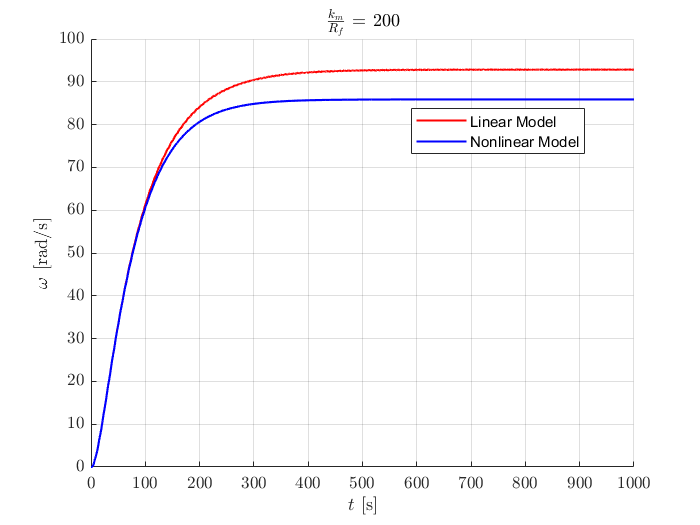
\includegraphics[scale = .5]{a200.png}
    \caption{Percent difference between linear and nonlinear model steady state is 7.8\%}
    \label{alpha200}
\end{figure}

\begin{figure}[h!]
    \centering
    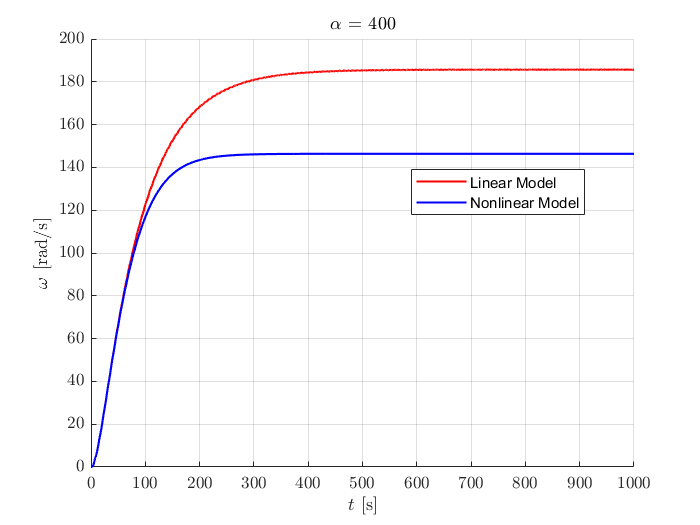
\includegraphics[scale = .5]{a400.png}
    \caption{Percent difference between linear and nonlinear model steady state is 23.7\%}
    \label{alpha400}
\end{figure}

\begin{figure}[h!]
    \centering
    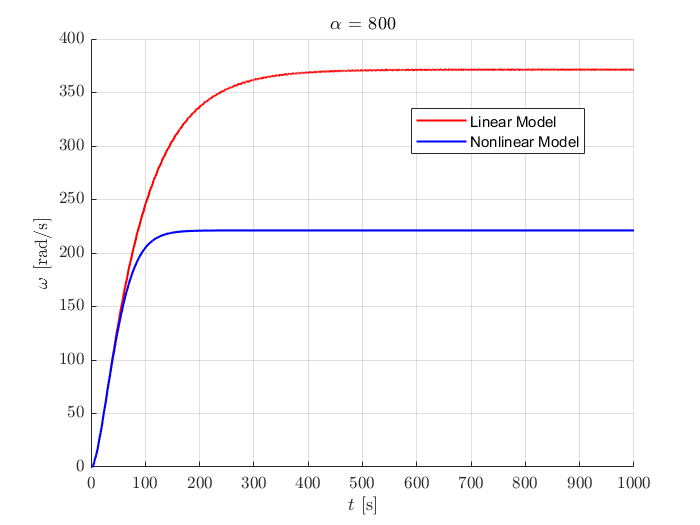
\includegraphics[scale = .5]{a800.png}
     \caption{Percent difference between linear and nonlinear model steady state is 50.7\%}
    \label{alpha800}
\end{figure}




\end{document}